%--------------------------------------------------------
%--------------------------------------------------------
\section{Generalized polarization operators and recovering standard power spectra}\label{sec:generalized_operators}  
With our better understanding of the radial part of the kernel for CMB polarization, we can write down generalized $E/B$-like fields that depend on a different radial function, even one that we specify to have compact support.
The spin symmetry constrains the the azimuthal part of the real space kernels to be of the form $\sim e^{\pm i2 \alpha}$.  The radial parts of the standard operators are determined by the sum over spherical harmonics and varies as a function of the band limit. It is here that we may potentially choose alternate forms for the radial functions to suit certain kind of analysis.

We can systematically generalize the real space operator by introducing the following harmonic space filter function:
%
\beq
\tilde{\mathcal{G}} = {\begin{bmatrix} g_{\ell}^E & 0  \\  0 & g_{\ell}^B \end{bmatrix}} \,,
\eeq
%
where the functions $g_{\ell}^E$ and $g_{\ell}^B$ represent the harmonic representation of the modified radial functions and can in the most general case be chosen to be different for $E$ and $B$ modes. To simplify discussions, we proceed by setting $g_{\ell}^E = g_{\ell}^B= g_{\ell}$. Given this harmonic function $g_{\ell}$, we can define the real space operator $\bar{O}'$ which translates Stokes $Q/U$ to $E/B$-like scalars (and the inverse operator $\bar{O}'^{-1}$) in the following manner,
% 
\begin{subequations} \label{eq:gen_qu2eb}
\beqry
{\bar O}' &=& {{}_0\mathcal{Y}} \, \tilde T^{-1} \tilde{\mathcal{G}} {{}_2\mathcal{Y}^{\ddag}} \, \bar T \,,\\
{\bar O}'^{-1}&=& \bar{T}^{-1} {{}_2\mathcal{Y}}\, \tilde{\mathcal{G}}^{-1} \tilde T {{}_0\mathcal{Y}^{\ddag}}.
\eeqry
\end{subequations}
%
The primed notation distinguishes these generalized operators from the default operators defined in \sec{sec:qu2eb} and \sec{sec:eb2qu}. We require both the forward and inverse operators to be well defined.   This constrains the choice of $\tilde{\mathcal{G}}$ to have a valid  inverse, which is important when recovering the standard CMB power spectra. The radial parts of this generalized operator and it's inverse are given by the following expressions,
%
\begin{subequations}\label{eq:generalized_radial_kernel}
\beqry 
G_{QU \rightarrow EB}(\beta) &=& G(\beta) = \sum _{\ell=2} ^{\ell_{\rm max}} g_{\ell}\frac{2 \ell+1}{4 \pi} \sqrt{\frac{(\ell-2)!}{(\ell + 2)!}} P_{\ell}^2(\cos{\beta}) \, \label{eq:mod_rad_forward} \,, \\
G_{EB \rightarrow QU}(\beta) &=& G^{-1}(\beta) = \sum _{\ell=2} ^{\ell_{\rm max}} g_{\ell}^{-1}\frac{2 \ell+1}{4 \pi} \sqrt{\frac{(\ell-2)!}{(\ell + 2)!}} P_{\ell}^2(\cos{\beta}) \,. \label{eq:mod_rad_inverse}
\eeqry
\end{subequations}
%
The default radial function is just a special case resulting from the choice $\tilde{\mathcal{G}}=\mathbb{1}$ ($g_{\ell}=1$), in which case $\tilde{\mathcal{G}}^{-1}=\tilde{\mathcal{G}}$ and therefore $G^{-1}(\beta) = G(\beta)={{}_{\mm}f}$.
%
\begin{figure}[!t] 
\centering
\subfigure[\label{fig:gl_gbeta}]{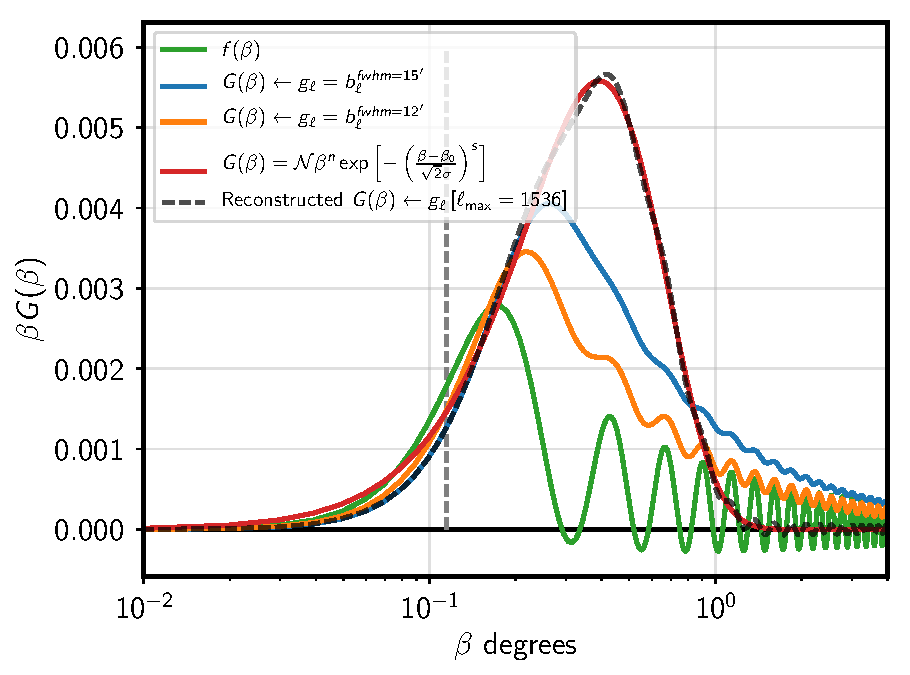
\includegraphics[width=0.48\columnwidth]{Gbeta_for_different_gl_lmax1536.pdf}}
\subfigure[\label{fig:glbl}]{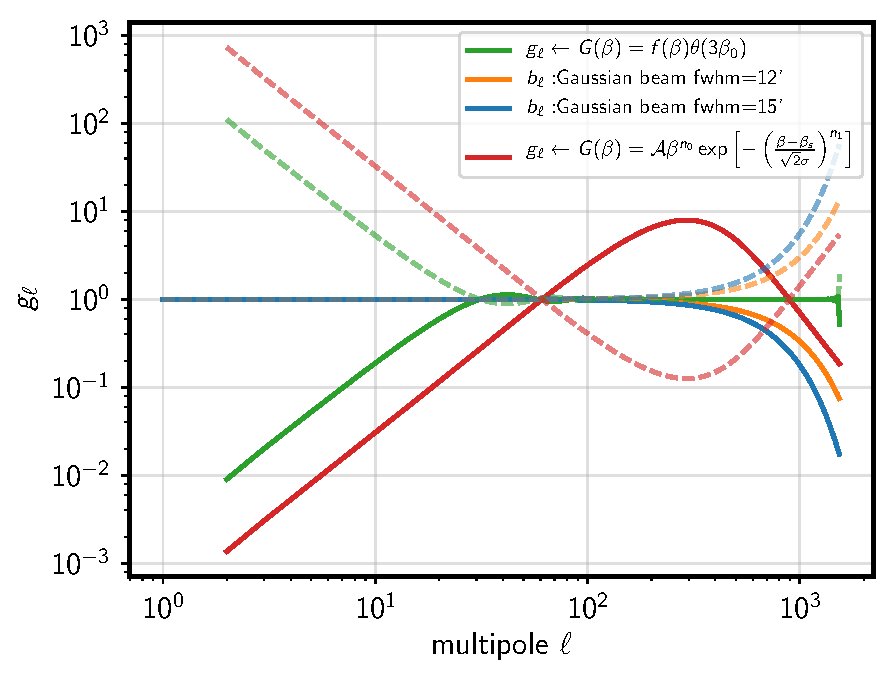
\includegraphics[width=0.48\columnwidth]{gl_for_different_gbeta_lmax1536.pdf}}
\subfigure[\label{fig:gl_bbeta}]{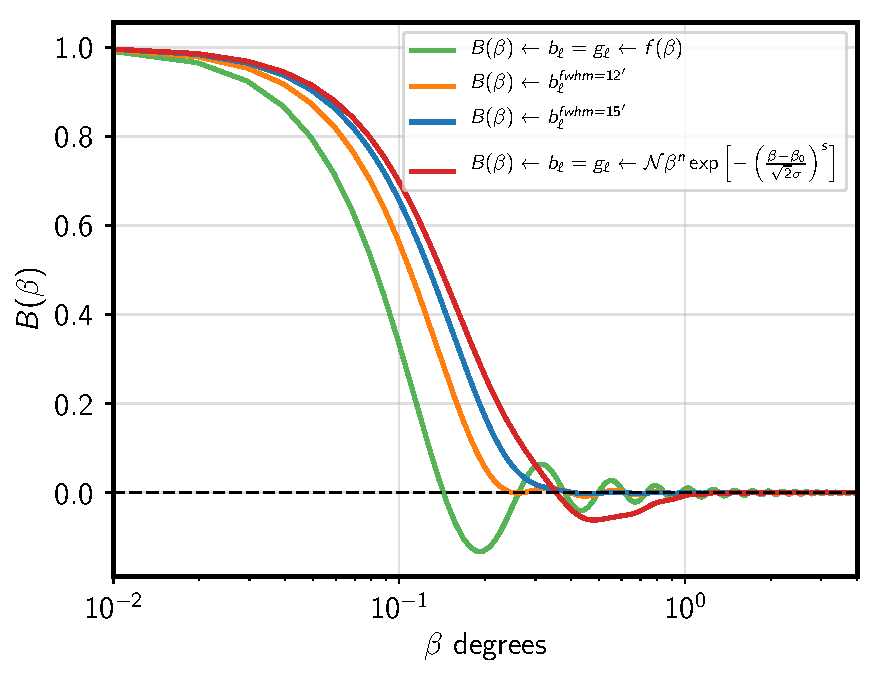
\includegraphics[width=0.48\columnwidth]{Bbeta_for_gl_lmax1536.pdf}}
\caption{\textit{Top left:} The green line depicts the default radial kernel $f(\beta)$ defined in \eq{eq:qu2eb_gen_kernel}, multiplied by an apodized step function $\theta(3 \beta_0)$. The blue and orange lines depict the modified radial function resulting the beam harmonics $b_{\ell}$ corresponding to Gaussian beams with fwhm=15 \& 12 arc-minutes respectively. The red curve depicts an example modified radial function: $G(\beta)=\mathcal{A} \beta^{n_o} \exp{\left[ -\left( {(\beta-\beta_s)}{/\sqrt{2} \sigma} \right)^{n_1} \right]}$ with parameters set to the following values $[n_0=1;\, \beta_s=0 ;\, \sigma = 0.004 ;\, n_1=1.5]$. The black dashed curve depicts the band limited reconstruction of the modified radial function. \textit{Top right:} The harmonic representation of the respective radial functions as indicated by the legend. The dashed curves of the corresponding color depict the inverse of the harmonic functions. \textit{Bottom:}  The normalized beam function $b(\beta)$ evaluated from interpreting the respective harmonic functions as those corresponding to an effective beam applied to $E/B$. }
\label{fig:example_gbeta}
\end{figure}
%

While defining these generalized operators, it is more natural to choose the real space function $G(\beta)$ rather than the harmonic space $g_l$, bearing in mind the constraint that $G(\beta=0)=G(\beta=\pi)=0$. Employing the orthogonality property of associated Legendre polynomials it can be shown that the harmonic function $g_{\ell}$ is given by the expression,
%
\beq
g_{\ell} = 2 \pi \sqrt{\frac{(\ell-2)!}{(\ell+2)!}} \int _{0}^{\pi} G(\beta) P_{\ell}^{2}(\cos{\beta}) d\cos{\beta} \,. \label{eq:gb2bl}
\eeq
%
An arbirtrary $G(\beta)$ for which $g_{\ell} \neq 1$ can be equivalently thought in terms of the standard $E/B$ fields being convolved with some effective circularly symmetric beam whose radial profile is given by the expression,
%
\beq
b(\beta) = \sum_{\ell=0}^{\ell_{\rm max}} \frac{2 \ell+1}{4 \pi} g_{\ell} P_{\ell}^{0} (\cos{\beta})\,,
\eeq
%
where $g_{\ell}$ is the same harmonic function as that appearing in \eq{eq:generalized_radial_kernel}.
In contrast to the radial function $G(\beta)$, a beam function when appropriately normalized has the property $b(\beta) \rightarrow 1$ as $\beta \rightarrow 0$. Though the real space functions $G(\beta)$ (operating on Stokes parameters) and $b(\beta)$ (operating on scalar $E/B$) are different, in harmonic space they play identical roles.

% Therefore it is possible to interpret the beam harmonic coefficients as those representing some modified radial kernel.
In \fig{fig:example_gbeta}, we examine in more detail the relationship between the modified radial kernels and these beam harmonic coefficients.  
 \fig{fig:gl_gbeta} depicts the radial profile of the  effective beams corresponding to different radial kernels: the standard kernel modified by a radial cutoff, kernels corresponding to Gaussian smoothings of the $E/B$ fields, and a radial function without oscillations and an exponential cutoff.  Note that the smoothing tend to increase the non-locality, indicated by the shifting right of the maxima of the respective kernels, as one may have expected.  The exponential cutoff (red curve) by construction has a very small non-locality (parameterized by $\beta_0$).

\fig{fig:glbl} depicts the harmonic description $g_{\ell}$ for these respective radial kernels and beams.
Finally, the beam that the modified radial kernels effectively apply to the $E/B$ fields are shown in \fig{fig:gl_bbeta}.  Note that the beam function corresponding to the default radial kernel ($g_{\ell}=1$) is merely a band limited representation of a delta-function beam.

The generalized convolution kernels defined in the previous section, when operated on the Stokes vector returns some scalar $E'$ and $B'$ mode maps,
%
\beq
\bar{S}' = \bar{O}' \bar{P}
\eeq
%
which are merely filtered versions of the standard $E/B$ modes maps. The filter function is simply $g_{\ell}$, which is easily obtained from the modified radial function $G(\beta)$.  It can be simply interpreted as the set of harmonic coefficients for some azimuthally symmetric beam. The power spectra of the modified scalar fields $E'$ and $B'$ are thus related to the spectra of the standard $E$ and $B$ fields via the following relation, 
 %
 \begin{subequations}
 \beqry
C_{\ell}^{EE,BB,EB} &= &C_{\ell}^{E'E',B'B',E'B'} /   g_{\ell}^2\,,\\
C_{\ell}^{TE,TB}  &=&  C_{\ell}^{TE',TB'} / g_{\ell}\,,
 \eeqry
 \end{subequations}
 %
 where $C_{\ell}$ denotes the angular power spectra and $T$ refers to the temperature anisotropy map. Therefore the standard CMB spectra can always be recovered as long as the $1/g_{\ell}$ and $1/g_{\ell}^2$ are well behaved functions, which can be ensured by making a suitable choice for the modified radial function $G(\beta)$. 
%--------------------------------------------------------

%--------------------------------------------------------
\paragraph{Relation to the spin raising $\eth^2$ and lowering $\bar{\eth}^2$ operators.}
Recall that on operating twice with the spin lowering operator on the Stokes charge ${}_{+2}X$ results in filtered version of $E/B$ maps as in \eq{eq:ebdef}. Now note that it is possible to construct a modified real space operator by choosing the harmonic space function to be $g_{\ell} = ({(\ell+2)!/(\ell-2)!})^{1/2}$, resulting in similarly filtered $E/B$ maps as follows:
%
\beq 
[\mathcal{E} + i \mathcal{B}](\hat{n}_e)=- \Delta \Omega\sum_{q=1}^{N_{\rm pix}} \Bigg\lbrace  \left[  \sum_{\ell=\ell_{\rm min}}^{\ell_{\rm max}} \frac{2 \ell+1}{4 \pi} P_{\ell}^2(\beta_{qe}) \right] e^{-i2\alpha_{eq}} {}_{+2}X(\hat{n}_{q}) \Bigg\rbrace \,. \label{eq:bl_ebdef_lower} 
\eeq
%
Comparing to \eq{eq:ebdef_lower} makes apparent the following mapping:
%
\beq
\bar{\eth}^2 \equiv \Delta \Omega \sum_{q=1}^{N_{\rm pix}} \left[ \sum_{\ell=\ell_{\rm min}}^{\ell_{\rm max}} \frac{2 \ell+1}{4 \pi} P_{\ell}^2(\beta_{qe}) \right] e^{-i2\alpha_{eq}}\,.
\eeq
%
The operator $\bar{\eth}^2$ is composed of derivative operations and hence has an implicit positional dependence for all numerical purposes which is made explicit in the band limited version of the operator.  The band limited version of the spin raising operator $\eth^2$ is derived by simply taking the conjugate of the above equation.
%--------------------------------------------------------
